\documentclass{beamer}
\usepackage{beamerthemeAmsterdam}
\usepackage{amsmath}
\usepackage{graphicx}
\usepackage{algpseudocode}
\usepackage{algorithmicx}
\usepackage{textcomp}

\iffalse
idee: alle slides uitwerken/kennen, en dan gewoon aan de klas vragen wat ze willen?
\fi

\newcommand{\lijstje}[1]{\begin{itemize} #1 \end{itemize}}

\title{Jpeg Compressie}
\subtitle{De Wondere Wereld van Wavelets}
\author{Jan Westerdiep \and Okke van Garderen}
\date{\today}
\institute{Universiteit van Amsterdam}

\renewcommand{\figurename}{}

\begin{document}

\frame{\titlepage}

\section{Recap}

\frame{\frametitle{Welk project bij wie?}
  \begin{columns}
    \begin{column}{0.5\textwidth}
      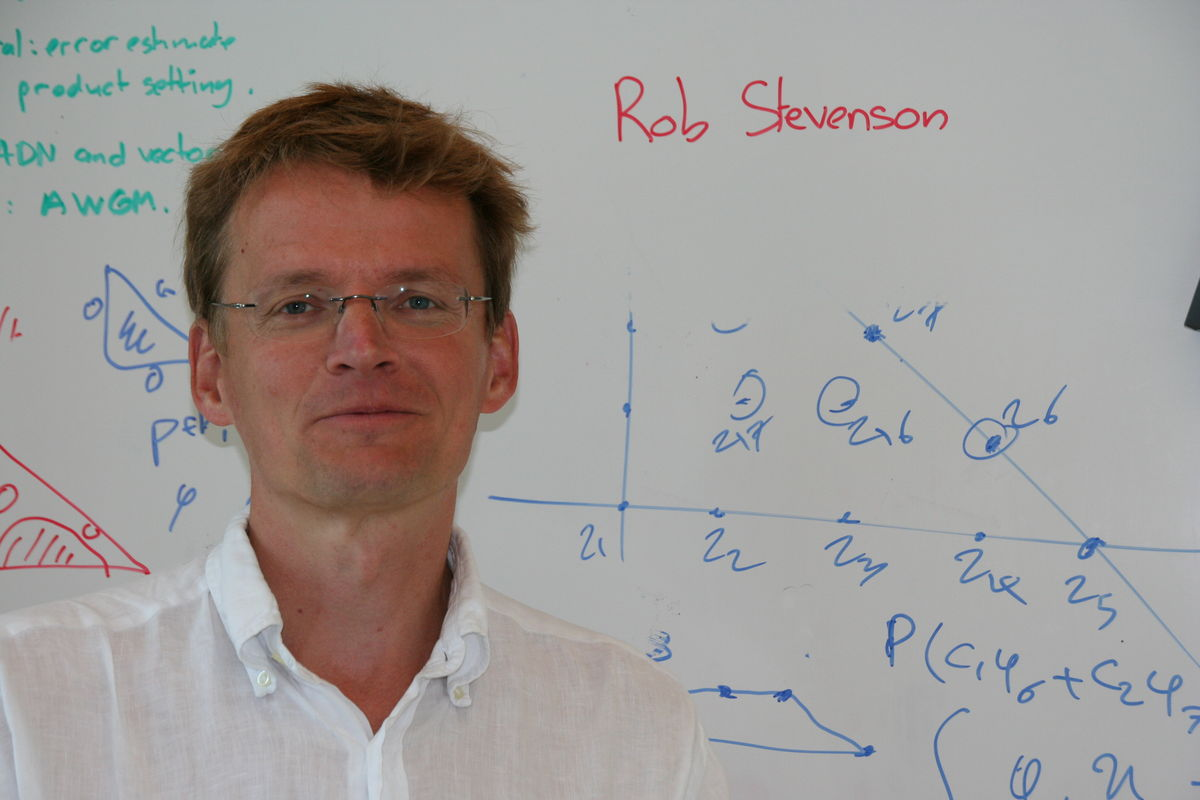
\includegraphics[width=\textwidth]{robbierobrob.jpg}
    \end{column}
    \begin{column}{0.5\textwidth}
      \lijstje{
        \item Rob Stevenson
        \item Compressie van signalen: Fouriertransformatie; Wavelettransformatie
        \item Lossy versus lossless
      }
    \end{column}
  \end{columns}
}

\section{Theoretische beschouwing}
\frame{\frametitle{Fouriertransformatie}
  \lijstje{
    \item Continu signaal $x(t)$, dan is de Fouriergetransformeerde:
    \[
      X(s) = \int_{-\infty}^\infty x(t) e^{-i 2 \pi s t} dt
    \]
    \item Probleem: calculus nodig, computer kan dit niet.
    \item Oplossing: DFT; transformeer signaal op bepaalde punten $\Rightarrow$ integraal wordt (eindige) sommatie
  }
}
\frame{\frametitle{DFT}
  \lijstje{
  \item $x_n$ is een lijst meetwaarden van lengte $N$
  \item De DFT hiervan geeft een nieuwe lijst $X_k$:
    \[
      X_k = \sum_{n=0}^{N-1} x_n \cdot e^{-i 2 \pi k n / N}
    \]
    \item !!! wanneer we te maken hebben met ``niet-continuiteit", kunnen we weinig/geen $X_k$'s weggooien
  \item $X_k$ is nu te beschouwen als de co\"effici\"ent van $k$'de basiselement
  \item inverse DFT:
    \[
      x_n = \frac{1}{N}\sum_{k=0}^{N-1} X_k \cdot e^{i 2 \pi k n / N}
    \]
  }
}
\iffalse
\frame{\frametitle{Uitleg}
  Keuze uit:
  \lijstje{
    \item is de inverse DFT ook echt een inverse
    \item voorbeeldje geven
  }
}
\fi
\frame{\frametitle{Voorbeeld}
  \lijstje{
  \item Stel $x = (0, 1, 0, -1)$
  \begin{align*}
    X_0 &= \sum x_n e^{-2 \pi i\cdot 0 \cdot n/4} = \sum x_n \cdot 1 = \sum x_n = 0 \\
    X_1 &= \sum x_n e^{-2 \pi i\cdot 1 \cdot n/4} = x_0 - i x_1 - x_2 + i x_3 = -\frac{1}{2}i \\
    X_2 &= \sum x_n e^{-2 \pi i\cdot 2 \cdot n/4} = x_0 - x_1 + x_2 - x_3 = 0 \\
    X_3 &= \sum x_n e^{-2 \pi i\cdot 3 \cdot n/4} = x_0 + i x_1 - x_2 - i x_3 = \frac{1}{2} i
  \end{align*}
  }
}
\frame{\frametitle{Voorbeeld}

  \lijstje{
  \item $x = (0,1,0,-1) \Rightarrow X = (0,-\frac{1}{2} i, 0, \frac{1}{2}i)$
  \item Hadden we dit ook anders kunnen zien?
  \[
    \sin(\pi x /2) \text{ op de punten } (0, 1, 2, 3)
  \]
  \[
    \sin( \pi x /2) = \frac{ e^{i \frac{1}{2} \pi x} - e^{- i \frac{1}{2} \pi x} }{2 i} = -\frac{1}{2}i e^{\frac{1}{2} i \pi x} + \frac{1}{2} i e^{-\frac{1}{2} i \pi x}
  \]
  \[
    = 0 + X_1 e^{\frac{1}{2} i \pi x} + 0 + X_3 e^{\frac{3}{2} \pi x} = \sum_{k=0}^{3} X_k e^{2 \pi i k x/4}!
  \]
  }
}

\frame{\frametitle{FFT}
  \small{
    \begin{algorithmic}
    \Function{FFT}{$x$}
    \State $n \gets \text{lengte}(x)$ \Comment Assumptie: $n$ is een tweemacht
    \If {$n == 1$}
      \State{$X \gets x$}
    \Else
      \State $E \gets FFT(x[0::2])$ \Comment{Pak alle even indices}
      \State $O \gets FFT(x[1::2])$ \Comment{Pak alle oneven indices}
      \For{$i = 0$ to $n-1$}
        \If{$i < n/2$}
          \State $X[i] \gets E[i] + e^{-2i \pi k/n} \cdot O[i]$
        \Else
          \State $X[i] \gets E[i] - e^{-2i \pi k/n} \cdot O[i]$
        \EndIf
      \EndFor
    \EndIf
    \State \Return{$X$}
    \EndFunction
    \end{algorithmic}
  }
}
\frame{\frametitle{Is deze FFT nou echt beter? Een les complexiteitstheorie}
\lijstje{
	\item Claim: DFT is $\mathcal{O}(n^2)$; FFT is $\mathcal{O}(n \log n)$
	\item Recurrente betrekking geeft aantal stappen van algoritme in formulevorm
	\[
		T(n) = \begin{cases}
		  c &\text{ als } n \leq d \\
		  a T(n/b) + f(n) &\text{ anders} \\
		\end{cases}
	\]
	\item (vereenvoudigde) stelling van Akra-Bazzi
	\[
		\exists k \in \mathbb{N}: f(n) \in \mathcal{O}(n^{\log a/\log b} \log^k n) 
	\]
	\[
		\Rightarrow T(n) \in \mathcal{O}(n^{\log a / \log b} \log^{k+1}n).
	\]
}
}

\frame{
\begin{columns}
\begin{column}{0.5\textwidth}
  \small{
    \begin{algorithmic}
    \Function{FFT}{$x$}
    \State $n \gets \text{lengte}(x)$
    \If {$n == 1$}
      \State{$X \gets x$}
    \Else
      \State $E \gets FFT(x[0::2])$
      \State $O \gets FFT(x[1::2])$
      \For{$i = 0$ to $n-1$}
        \If{$i < n/2$}
          \State $X[i] \gets E[i] + e^{-2i \pi k/n} \cdot O[i]$
        \Else
          \State $X[i] \gets E[i] - e^{-2i \pi k/n} \cdot O[i]$
        \EndIf
      \EndFor
    \EndIf
    \State \Return{$X$}
    \EndFunction
    \end{algorithmic}
  }
\end{column}
\begin{column}{0.6\textwidth}
	\[
		T(n) = \begin{cases}
		  c &\text{ als } n \leq d \\
		  a T(n/b) + f(n) &\text{ anders} \\
		\end{cases}
	\]
	\[
		\exists k \in \mathbb{N}: f(n) \in \mathcal{O}(n^{\log a/\log b} \log^k n) 
	\]
	\[
		\Rightarrow T(n) \in \mathcal{O}(n^{\log a / \log b} \log^{k+1}n).
	\]
	We vinden
	\[
		c=1; a=2; b=2;
	\]
	\[
		f(n) \in \mathcal{O}(n) = \mathcal{O}(n^1 \log^0 n)
	\]
	\[
		\Rightarrow \text{FFT} \in \mathcal{O}(n^1\log^1) = \mathcal{O}(n \log n)
	\]
\end{column}
\end{columns}

}

\section{Resultaten}
\frame{\frametitle{1 Kanaals - 1D Geluid}
  \lijstje{ 
  \item[?] spongebob.wav
  \item[?] pokemon.wav
  }
}
\frame{\frametitle{1 Kanaals - 2D plaatjes}
\lijstje{
	\item 1 kanaal: matrix van grijswaarden: hoe hoger, hoe lichter
}
\begin{columns}
	\begin{column}{.5\textwidth}
	  
\includegraphics[width=\textwidth]{plaatje.jpg}% picture filename
	\end{column}
	\begin{column}{.5\textwidth}
	  $\left[ \begin{array}{rrrrrr}
		250 & 237 & 215 & 209 & 218 & 238 \\
		237 & 194 & 138 & 109 & 136 & 195 \\
		217 & 133 &  45 &  15 &  46 & 135 \\
		204 & 103 &  14 &   0 &  14 & 105 \\
		215 & 128 &  36 &  11 &  38 & 128 \\
		233 & 186 & 120 &  91 & 120 & 185 \\
	  \end{array}\right]$
	\end{column}
\end{columns}
}
\frame{\frametitle{4 Kanaals - 2D plaatjes}
\begin{columns}
	\begin{column}{.5\textwidth}
		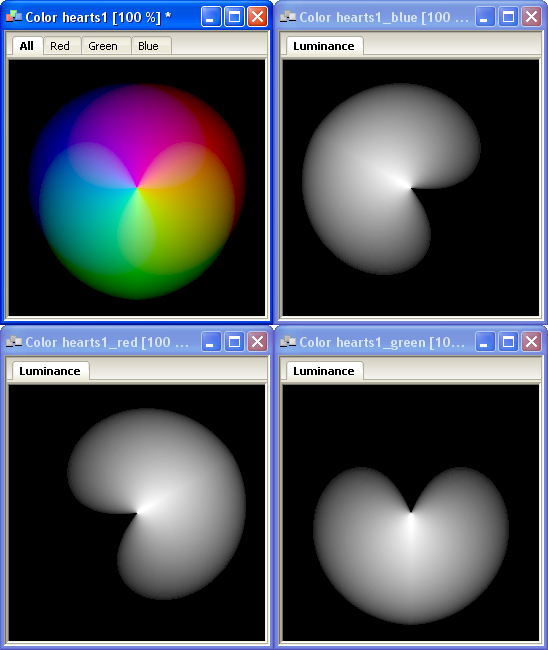
\includegraphics[width=\textwidth]{splitchannels.jpg}% picture filename
	\end{column}
	\begin{column}{.5\textwidth}
		\lijstje{
			\item 3 kleurenkanalen: Rood, Groen, Blauw
			\item Mogelijk 1 extra alpha-kanaal
			\item Hogere waarde $\Rightarrow$ pixel bevat meer kleur van die component
		}
	\end{column}
\end{columns}
}

\frame{
  \begin{figure}
    
\includegraphics[height=0.8\textheight]{presi_plaatjes/gentoo.png}
    \caption{Originele plaatje}
  \end{figure}
}
\frame{
  \begin{figure}
    
\includegraphics[height=0.8\textheight]{presi_plaatjes/gentoo_new_60p.png}
    \caption{60\% data}
  \end{figure}
}
\frame{
  \begin{figure}
    
\includegraphics[height=0.8\textheight]{presi_plaatjes/gentoo_new_8p.png}
    \caption{8\% data}
  \end{figure}
}
\frame{
  \begin{figure}
    
\includegraphics[height=0.8\textheight]{presi_plaatjes/gentoo_new_2p.png}
    \caption{2\% data}
  \end{figure}
}
\frame{
  \begin{figure}
    
\includegraphics[height=0.8\textheight]{presi_plaatjes/gentoo_new_0_5p.png}
    \caption{5\textperthousand data}
  \end{figure}
}

\section{Toekomst}
\frame{\frametitle{Toekomst}
  \lijstje{
  \item Overschakelen naar Wavelets
  \item 3D / Filmpjes
  }
}

\section{Slides voor Chris}
\frame{
  \lijstje{
  \item Volgende slides geven antwoord op Chris zn vragen
  }
}

\frame{
Voorbeeldvraag:
- waarom zou je uberhaupt FFT doen
- significantie coeffs (toepassing babyvoorbeeld)
- FFT op plaatje (2d fft), hoe werkt het? -> FFT op rijen van plaatje, dan FFT op kolommen van je FFT (ofzo?)
}

\end{document}
